
%% Warning: section is very new, and likely subject to errors
% TODO: double-check correctness of new code.
% TODO: proofread


\subsection{Integrals}\label{sec:integrals}
Say we've got a function. This function can be expressed as a line on a graph. This line separates the graph in two sections; one above and one below the line.

\begin{figure}[h!]
    \centering
    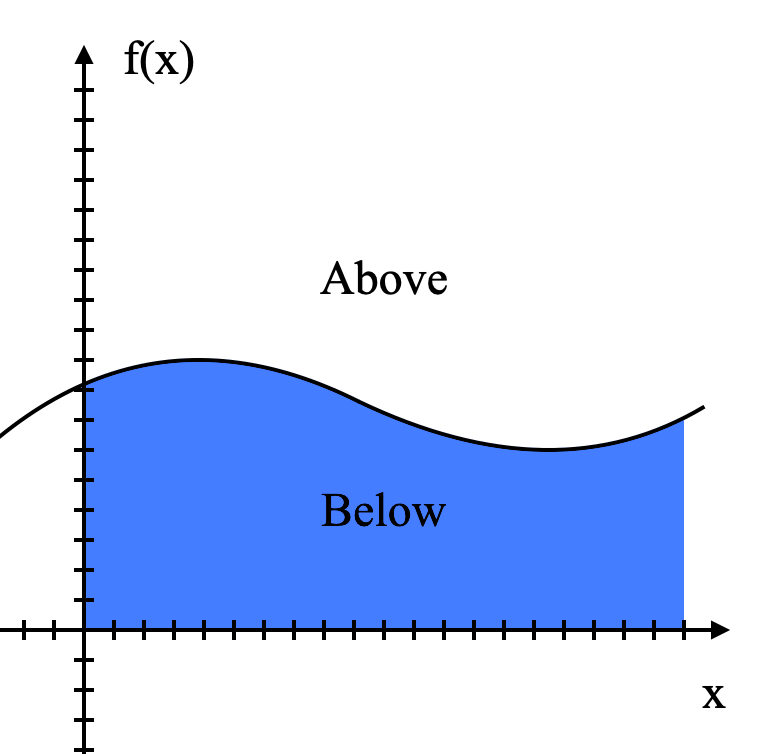
\includegraphics[scale= 0.3]{Images/integralGraph.png}
    \caption{}
    \label{integralgraph}
\end{figure}

How much space exists below the line?

\subsubsection{Setting up the Language}
A problem like the one described above is normally solved with an integral. To solve an integral, we'll first need a language that can describe the function(which in turn describes the line).

Unlike complex numbers, there is no one uniform expression that can describe any function. Polynomials, however, get pretty close, so let's use those as a basis:
%Thus, this time, we'll have to invent something a little bit more flexible.

\iffalse
\begin{minted}{haskell}
data Funk = X
  | Constant Double
  | Add Funk Funk
  | Multiply Funk Funk
  deriving (Show)
\end{minted}
\fi
\begin{minted}{haskell}
data Funk =
  | Constant Double
  | X Double
  | XSquare Double
  | Add Funk Funk
  deriving (Show)
\end{minted}

The essence of polynomials is to split an expression into smaller chunks that are added together to create a greater whole. Each line in the above datatype is a ''word'' in our DSL. The constant should be self-explanatory; it's a constant number, expressed as a Double. ''X Double'' is our way of writing basic undefined variables on the form ''aX'', I.E. 5X, 0.33X, or indeed just 1X. XSquare uses the same basic concept; ''aX$^2$'' can be 5X$^2$, 0.33X$^2$, etc.
Finally, ''Add'' is used to string our words together into ''sentences''. As an example, the polynomial function ''$5 + 4X^2$'' would in our DSL be written as
\begin{minted}{haskell}
test :: Funk
test = Add test1 test2 where
    test1 = Constant 5
    test2 = XSquare 4
\end{minted}

Simple enough, and easily expanded, too. If we ever wanted any other functionality, be it roots, pies, or trigonometric functions, we'd simply need to add a word for them. As such, we can keep our ''language'' limited to the above for now; the rest will be added in the sections that use them.

\iffalse
We'll do something a little more standard this time. The above DSL mimics the standard syntax for functions, or at least as closely as we can make it. Our ''words'' are the variable X, a constant, addition, and multiplication.

These are theoretically used in the exact same way that they would be on paper; the first two are values, while the second two are operators. For simplicity's sake, we'll be using an integer to describe our constants. X is, as you'd expect, an undefined variable.

Our operators; addition and multiplication, are a little more complicated. Rather than being simple values, they are statements that take other ''words'' and tie them together. Perhaps this is best explained by an example. Say you want the function ''$5 + x^2$''. In our DSL, we'd write it as
\begin{minted}{haskell}
test :: Funk
test = Add test1 test2 where 
            test1 = Constant 5
            test2 = Multiply X X
\end{minted}

The Multiply word, in this case, ties two X's together, while the Add word ties the result to the constant. Thus, we've created a ''sentence'' of words(or a function, according to math).

This is still a very limited language. At some point, we'll probably want more words to describe any other operations we might want to be part of our calculations; powers, divisions, roots, etc. The list is effectively endless, and so to keep things comprehensive, let's stick to this simplified version for now.
\fi

\paragraph{} We're still not ready for integrals, however. First, we'll also need a function that takes the sentences(functions) we just created and calculates them to produce a result. In practice, this is simplicity itself; we'll simply replace each word with their algebraic equivalent and let Haskell roleplay as a calculator for a moment. To wit:
\begin{minted}{haskell}
-- calculate
--input: function, value for X
--output: result
calculate :: Funk -> Double -> Double
calculate (Constant double) value = double
calculate (X double) value        = double * value
calculate (XSquare double) value  = double*(value^2)
calculate (Add funk1 funk2) value = (calculate funk1 value) + (calculate funk2 value)
\end{minted}

As noted in the code itself, the ''value'' input is whichever value we desire X to be.

\begin{exercise}
Expand the DSL with a word for powers other than squares. Like the other words, it should include a constant multiplier and integrate correctly with ''calculate'', above. Hint: as evidenced by Add, there is no rule saying a word can only include one value.
\end{exercise}

\iffalse
\begin{minted}{haskell}
-- calculate
--input: function, value for X
--output: result
calculate :: Funk -> Double -> Double
calculate X value                       = value
calculate (Constant num) value          = num
calculate (Add funk1 funk2) value       = (calculate funk1 value) + (calculate funk2 value)
calculate (Multiply funk1 funk2) value  = (calculate funk1 value) * (calculate funk2 value)
\end{minted}

\begin{exercise}
Expand the DSL with a word for subtraction, and full functionality in the 'Calculate' operator. 
\end{exercise}
\fi

\subsubsection{Brute Force Mathematics}
Right, with our basic language defined, it's time to take a first stab at that graph.

The traditional first step to solving an integral is to, instead of look for an entirely accurate answer, instead look for an estimated answer.

To wit, let's use our test function from above (5 + $4x^2$), and say we want to know how much space exists beneath the line and between x=2 and x=5. To do this, we could take the average of these numbers, (2+5)/2=3.5, and see how much space would exist between the line if this average was true throughout the function.
\begin{minted}{haskell}
-- bfIntegral (brute force integral)
--input: function, startvalue, stopvalue
--output: result
bfIntegral :: Funk -> Double -> Double -> Double
bfIntegral funk start stop = (calculate funk ((start+stop)/2)) * (stop-start)
\end{minted}

There, quick and easy. Sadly not accurate. Our main problem is that our test function does not grow linearly. This means that taking a value ''in the middle'' of the graph and expecting the values on either side to balance each other out is foolish.

Rather than despair, however, let's try to make our integral a little more accurate. The way we go about this is that rather than use an average for the entire graph, we cut the problem into equally sized chunks, calculate each chunk individually, and add the results together.

\begin{figure}[h!]
    \centering
    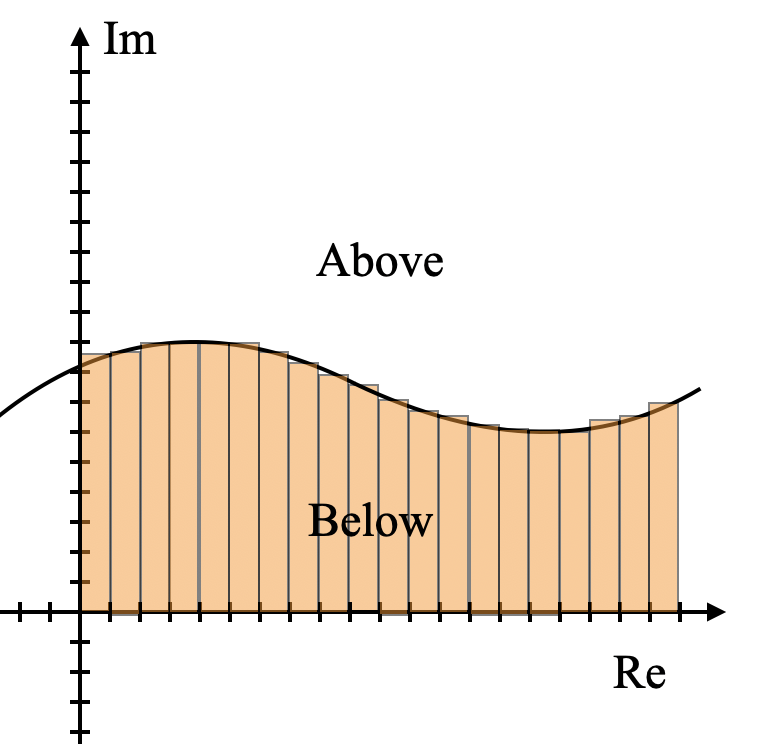
\includegraphics[scale= 0.5]{Images/integralBruteForce.png}
    \caption{}
    \label{integralbruteforce}
\end{figure}

\begin{minted}{haskell}
-- bfIntegral' (brute force integral alternative)
--input: function, start, end
--output: result
bfIntegral' :: Funk -> Double -> Double -> Double
bfIntegral' funk start end
  | start >= end = 0
  | otherwise    = (calculate funk start) + (bfIntegral' funk (start+1) end)
\end{minted}
We made each chunk precisely 1 wide for simplicity, using a simple recursive function. The result should be considerably more accurate now, though still not perfect.

We also learnt an important lesson. See, the first example used chunks as well. Or rather, a single chunk. By cutting the chunk into smaller chunks, we increased accuracy. This is something we can repeat. In theory, we can repeat it infinitely; cutting our problem into an infinite number of infinitely small chunks. If each size reduction on the part of the chunks brings us closer to the true answer, and we reduce the size infinitely, then we will become infinitely close to the true answer. I.E. We will have the true answer.

\paragraph{} In practice, no computer can actually calculate infinity, but they can get close enough for most purposes. So let's give that a shot and see what happens;
\begin{exercise}
Create a version of the brute-force Integral operator that uses 100 times the width worth of chunks.

\cmd{bfIntegral'' :: Funk -> Double -> Double -> Double}\\
\cmd{-- bfIntegral'' (brute force integral: electric boogaloo)}\\
\cmd{--input: function, start, stop}\\
\cmd{--output: result}
\end{exercise}
\iffalse
let's make one chunk for every 1/100.
\begin{minted}{haskell}
-- bfIntegral'' (brute force integral: electric boogaloo)
--input: function, start, stop
--output: result
bfIntegral'' :: Funk -> Double -> Double -> Double
bfIntegral'' funk start end
  | start >= end = 0
  | otherwise    = (calculate funk start)*0.01 + (bfIntegral'' funk (start+0.01) end)
\end{minted}
\fi

 If this is still not enough.. well, there's still one subsection left to read. Beware though, it'll require a little more mathematical understanding.

\subsubsection{An Elegant yet Primitive Solution}
*deep breath*

During prior math courses, you should've ran into derivative functions.

A derivative function, conceptually speaking, is a function transformed from describing a value for a specific input, to describing how that value changes depending on input.

You may realize that this sounds eerily similar to what we are hoping to do with integrals; let's take another look at the graph from the beginning of this section \ref{integralgraph}.


We are looking for the value underneath the line described by a function; a line that describes the change in that value depending on input. We are looking for the exact opposite of a derivative function. We are looking for what mathematicians refer to as ''primitive functions''. This name is an homage to the idea that our function has already been derived, and we are seeking its ancient, gnarled, ''primitive'' ancestor. In this manner, all functions can be considered to exist in secret pairs; a primitive ancestor, and a punk derivative.

For the sake of brevity, let's not go indepth on how derivativation function on a micro-level, and instead limit ourselves to the more commonly used laws of derivation. Specifically, let's invert them:

\begin{minted}{haskell}
primitivize :: Funk -> Double -> Funk
primitivize funk constant = Add (primitivize' funk) + (Constant constant)

primitivize' :: Funk -> Funk
primitivize' Constant double = X double
primitivize' X double        = XSquare (double/2)
primitivize' XSquare double  = -- Your implementation of powers goes here; power=3, double/3
primitivize' Add funk1 funk2 = Add (primitivize' funk1) (primitivize' funk2)
\end{minted}

Assuming the rules of derivation are known, the bulk of primitivize' shouldn't be overly surprising.
When deriving, each X is multiplied with their power, and then said power is reduced by one. Thus, if we're seeking the primitive function version of the function, we instead increase the power by one, and then divide by the new power.
Standalone constants are removed when deriving. Thus, any remaining constants in derived version of the function must've once had an attached variable.
In addition, we must consider the possibility that there once was another constant that was lost on derivation; this is why we must supply a replacement constant when finding the primitive function. For integral purposes, this constant will always be zero, but it's still important to know that it technically exists.
Add remains unchanged.

Going back to the example used in the brute force solution, we should now be able to get a perfect answer:
\begin{minted}{haskell}
primitiveTest :: Funk
primitiveTest = primitivize test 0
calculate ((primitiveTest 5) - (primitiveTest 2))
\end{minted}

\begin{exercise}
Extend support for other powers to this form of integral.
\end{exercise}
\begin{exercise}
ADVANCED: Expand the DSL with a word for a complex constant, plus associated functionality for both types of integral.
\end{exercise}

Once set up, the primitive solution is indeed elegant, but it does have one major flaw; it only works so long as we can find a primitive version of the function, and depending on the operators involved, this might be easier said than done.

Finally, there are more extensive versions of the above haskell code in the appendix, if you're interested.